%!TEX TS-program = pdflatex
%!TEX encoding = UTF-8 Unicode
%!TEX spellcheck = English (Aspell)

\documentclass[11pt]{article}
\usepackage{lucy,handout,graphicx,tikz}

% =========================================================
\begin{document}


\noindent 
Suppose you decide to organize a Snakes and Ladders competition with $n$
participants. In this competition, each game of Snakes and Ladders involves
three players. After the game is finished, they are ranked first, second, and
third.  Each player may be involved in any (non-negative) number of games, and
the number need not be equal among players.

At the end of the competition, $m$ games have been played.  You realize that you
forgot to implement a proper rating system, and therefore decide to produce the
overall ranking of all $n$ players as you see fit.  However, to avoid being too
suspicious, if player $A$ ranked better than player $B$ in at least one game,
then $A$ must rank better than $B$ in the overall ranking.

You are given the list of players and their rankings in each of the $m$ games.
Describe and analyze an algorithm that produces an overall ranking of the $n$
players that is consistent with the individual game rankings, or correctly
reports that no such ranking exists.

\begin{enumerate}
    \item It is always good practice to come up with an example to make sure you
    understand the problem statement. Give an example competition with four
    distinct players and the outcome of three games. Propose an overall ranking of the players.
    Is it valid?
    \begin{Solution}
    Let's say the players are $p_1, p_2, p_3, p_4$, and they play the following games:
    \begin{itemize}
        \item Game 1: $p_2$ first, $p_3$ second, $p_1$ third
        \item Game 2: $p_3$ first, $p_1$ second, $p_2$ third
        \item Game 3: $p_2$ first, $p_4$ second, $p_3$ third
    \end{itemize}
    Let's ask whether $p_1, p_2, p_3, p_4$ is a valid ranking.  We can see that
    the answer is \EMPH{no}, because $p_4$ ranked above $p_3$ in game 3, but
    $p_4$ does not rank better than $p_3$ in the overall ranking.
    \end{Solution}
    \item Your algorithm must be a reduction to a graph problem. Draw the graph
    you would build for your instance and use it to demonstrate that your overall ranking
    is or is not valid.
    \begin{Solution}
    The graph has one vertex for each player.  For each game, we add a directed
    edge from every higher-ranked player to every lower-ranked player in that game:
    \[
    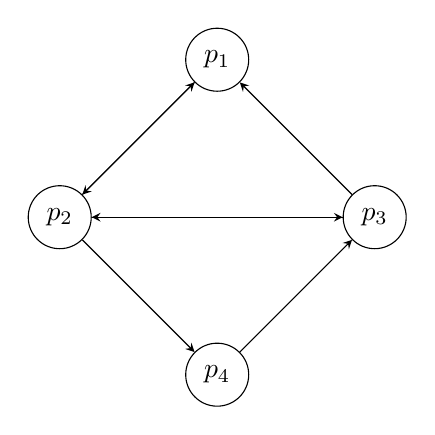
\begin{tikzpicture}[
        player/.style={circle, draw, minimum size=8mm, inner sep=0pt},
        >=stealth,
        every edge/.style={draw, ->},
        edge label/.style={font=\scriptsize, fill=white, inner sep=1pt}
    ]
        \node[player] (p1) at (0,2) {$p_1$};
        \node[player] (p2) at (-2,0) {$p_2$};
        \node[player] (p3) at (2,0) {$p_3$};
        \node[player] (p4) at (0,-2) {$p_4$};

        \path (p2) edge  (p3)
                    edge  (p1)
                    edge  (p4);
        \path (p3) edge  (p1)
                    edge (p2);
        \path (p1) edge  (p2);
        \path (p4) edge  (p3);
    \end{tikzpicture}
    \]
    The graph contains the directed cycle
    $p_1\mathbin{\to}p_2\mathbin{\to}p_1$, so it has no topological ordering.
    Therefore, no overall ranking can satisfy all of the game constraints; in
    particular, the proposed ranking $p_1,p_2,p_3,p_4$ is not valid.
    \end{Solution}

    \item You are now ready to write down your full algorithm. You can do so by answering the following questions:
\begin{itemize}
\item What are the original parameters of the problem? (That is, the variables
describing the input?) You will need this to analyze the runtime of your
algorithm.
\begin{Solution}
    $n$ players and $m$ games.
\end{Solution}
\item What are the vertices?  What does each vertex represent?
\begin{Solution}
    There is one vertex per player.
\end{Solution}
\item What are the edges?  Are they directed or undirected?
\begin{Solution}
    A directed edge exists between $p_i$ and $p_j$ if $p_j$ ranked higher than $p_i$
    in some game.
\end{Solution}
\item If the vertices and/or edges have associated values, what are they?
\begin{Solution}
    None needed.
\end{Solution}
\item \textbf{What is the precise relationship between your graph and the stated problem?}
\begin{Solution}
Any topological order of the vertices is a valid ranking, since no
player can come before another in the toplogical order if they beat them
in some game. If the graph has a cycle, then there is no toplogical order,
and there is no valid ranking.
\end{Solution}
\item What standard graph algorithm are you using to solve the problem?
\begin{Solution}
It would be okay to just say ``check for cycles and compute a topological order'',
but to be more specific,
we can run DFS recording post order values. If there is any edge $a\to b$ so that $a.post > b.post$,
there is a cycle, and we can say there is no valid ranking. Otherwise, return the nodes in reverse
post order.
\end{Solution}
\item What is the running time of your entire algorithm, \emph{including} the time to build the graph, \emph{as a function of the original input parameters}?
\begin{Solution}
    The graph has $n$ vertices and $O(m)$ edges, since
    each game contributes up to 3 edges, so $V=n$ and $E=O(m)$. DFS takes $O(V+E)$
    time and the brute-force check of edges takes $O(E)$ time. Returning a reverse
    post order of the vertices takes $O(V)$ time. Therefore, the overall runtime is
    $O(V+E)$, which is $O(n+m)$ in terms of the original parameters of the problem.
\end{Solution}
\end{itemize}
\end{enumerate}


%----------------------------------------------------------------------


\end{document}